% =============================================================================
% Section 3 — System Architecture
% Source-extracted from repository: 2026-08-05
%   poc-gesture-detector.ts          (state machine, EAR constants)
%   DetectionProfileService.java      (profile publish, versioning)
%   ReportIngressService.java         (12-step ingestion pipeline)
%   V1__gest_poc_schema.sql           (GEST domain schema)
%   poc/V1__evnt_poc_schema.sql       (EVNT event schema)
% =============================================================================

\section{System Architecture}
\label{sec:architecture}

NeuroAssist AI is composed of two deployable contexts: a~\emph{browser-side detection
pipeline} executed entirely within the patient's device, and a~\emph{backend alert
pipeline} implemented as hexagonal microservices. Figure~\ref{fig:overview} illustrates
the end-to-end data flow.

% ─── 3.1 System Overview ──────────────────────────────────────────────────────
\subsection{System Overview}
\label{sec:overview}

The pipeline is triggered by a~deliberate facial gesture captured by any commodity
webcam (720\,p or higher). The gesture detection loop runs exclusively in the browser
via WebAssembly; no video frames leave the device at any point. When a~gesture is
confirmed by the state machine (Section~\ref{sec:statemachine}), a~lightweight JSON
payload is POSTed to the event ingestion service. The service validates the gesture
against the patient's active detection profile, creates an \texttt{Evento} record, and
dispatches a~\texttt{FULL\_SCREEN\_ALARM} notification. A caregiver application polls
the backend every five seconds; upon detecting an active event it renders a~full-screen
alarm overlay. The caregiver confirms attendance, which writes a~\texttt{verdict} back
to the event record and clears the alarm.

\begin{figure}[htbp]
  \centering
  % Replace with exported PDF from fig_sequence.mmd
  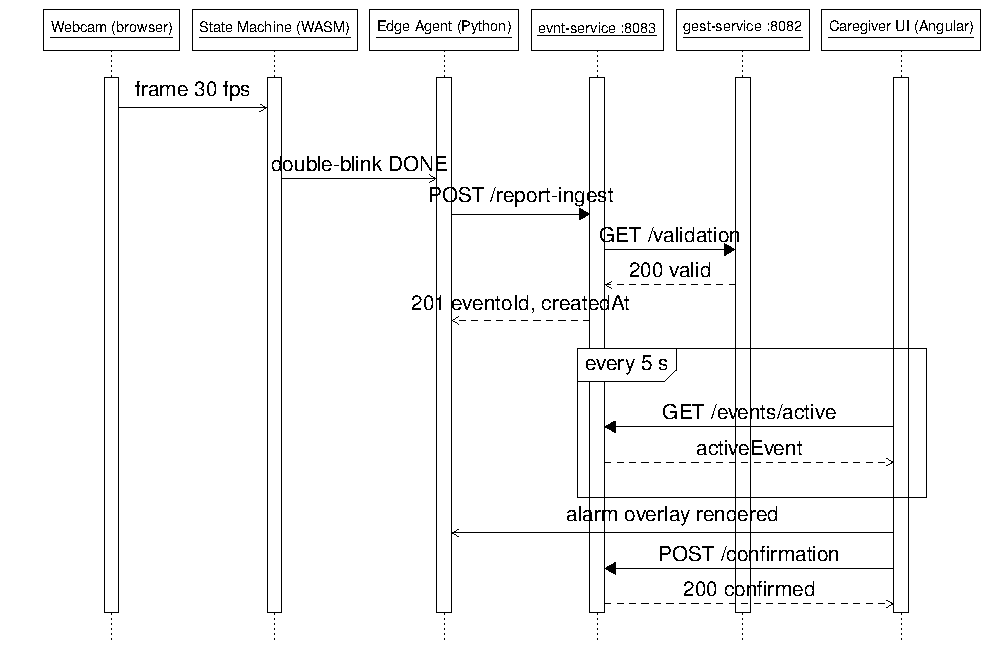
\includegraphics[width=\columnwidth]{figures/fig_overview}
  \caption{End-to-end data flow. Video is processed entirely in the browser
    (WASM); only structured JSON reports cross the network boundary.}
  \label{fig:overview}
\end{figure}

% ─── 3.2 Offline-First Gesture Detection ──────────────────────────────────────
\subsection{Offline-First Gesture Detection}
\label{sec:detection}

Facial landmark extraction is performed by MediaPipe
FaceLandmarker~\cite{lugaresi2019mediapipe} running on the CPU WebAssembly delegate.
The WASM binary and the \texttt{float16} face landmarker model are bundled as static
assets and served from \texttt{/assets/mediapipe-wasm/}; there is no dependency on any
content delivery network during gesture detection. The model download of approximately
30\,MB occurs once on first use and is thereafter served from the browser cache.

The landmarker produces 468 normalised landmarks per frame in a~\texttt{requestAnimation\-Frame} loop
running at approximately 30\,fps. Each frame yields:
\begin{enumerate}
  \item \textbf{EAR (Eye Aspect Ratio)} for each eye, computed from six landmarks
    \{33, 160, 158, 133, 153, 144\} (left) and \{362, 385, 387, 263, 373, 380\}
    (right) using the formulation of Soukupov{\'a} and {\v{C}}ech~\cite{soukupova2016}:
    \begin{equation}
      \text{EAR} = \frac{\|p_2 - p_6\| + \|p_3 - p_5\|}{2 \cdot \|p_1 - p_4\|}
      \label{eq:ear}
    \end{equation}
    where $p_1$--$p_6$ are the six eye landmarks in order.
  \item \textbf{Blendshape scores} (\texttt{eyeBlinkLeft}, \texttt{eyeBlinkRight},
    \texttt{browInnerUp}, \texttt{browOuterUpLeft}, \texttt{browOuterUpRight}) in $[0,1]$,
    used for single-eye blink and eyebrow raise detection.
\end{enumerate}

The system supports six gesture types: double blink (EAR-based), left and right individual
eye blink (blendshape-based), and bilateral or unilateral eyebrow raise
(blendshape-based). A shared 4\,s cooldown timer prevents duplicate firing across all
gesture types.

% ─── 3.3 Six-State Deliberate Gesture State Machine ──────────────────────────
\subsection{Six-State Deliberate Gesture State Machine}
\label{sec:statemachine}

The primary gesture — double blink — is disambiguated from involuntary blinks through a
six-state finite automaton shown in Figure~\ref{fig:statemachine}. Natural involuntary
blinks last 100--400\,ms and occur at 15--20 events per minute~\cite{bentivoglio1997}; the
state machine rejects spurious closures that do not meet minimum-duration requirements.

The six states and their transition conditions (all thresholds are patient-configurable
via the detection profile, Section~\ref{sec:calibration}) are as follows:

\begin{enumerate}
  \item \textbf{WAITING\_BLINK1}: idle. Transition to \textsc{in\_blink1} when
    $\text{EAR}_\text{avg} < 0.20$ ($\theta_\text{close}$).
  \item \textbf{IN\_BLINK1}: counting closed frames. Accept first blink and advance to
    \textsc{waiting\_open1} when the eye reopens ($\text{EAR}_\text{avg} \geq 0.27$,
    $\theta_\text{open}$) \emph{after} at least $f_\text{min}{=}3$ consecutive closed
    frames (${\approx}100$\,ms at 30\,fps); otherwise reject and return to
    \textsc{waiting\_blink1}.
  \item \textbf{WAITING\_OPEN1}: verifying full re-opening. Advance to
    \textsc{waiting\_blink2} after $f_\text{open}{=}3$ consecutive open frames; records
    timestamp $t_1$.
  \item \textbf{WAITING\_BLINK2}: awaiting second blink onset, subject to a timeout:
    if $\Delta t = \text{now} - t_1 > 1800$\,ms ($T_w$), the automaton resets to
    \textsc{waiting\_blink1}.
  \item \textbf{IN\_BLINK2}: counting second blink closed frames. Accept and advance to
    \textsc{done} when eye reopens with $f_\text{count} \geq 3$ and $\Delta t \leq T_w$;
    otherwise reject and reset.
  \item \textbf{DONE}: gesture confirmed; fires event, resets all state, enters 4\,s
    cooldown.
\end{enumerate}

\begin{figure}[htbp]
  \centering
  % Replace with exported PDF from fig_statemachine.mmd
  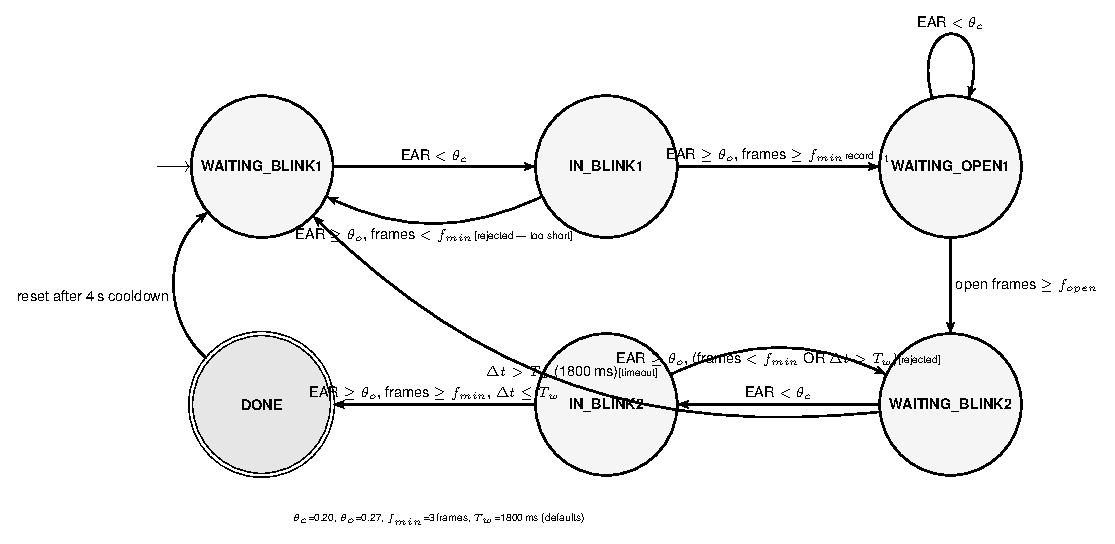
\includegraphics[width=\columnwidth]{figures/fig_statemachine}
  \caption{Six-state deliberate double-blink state machine. Dashed transitions
    indicate rejection paths that reset the automaton. $\theta_c{=}0.20$,
    $\theta_o{=}0.27$, $f_\text{min}{=}3$\,frames, $T_w{=}1800$\,ms.}
  \label{fig:statemachine}
\end{figure}

The requirement for minimum closure duration ($f_\text{min}$) in \emph{both} blinks,
combined with mandatory full re-opening in \textsc{waiting\_open1} and a~temporal
window $T_w$, collectively prevent the three principal sources of false positives in
residual-movement populations: single involuntary blinks, partial closures (e.g., ptosis
artefacts), and slow drift that crosses the threshold without a~discrete blink.

% ─── 3.4 Patient Calibration (DetectionProfile) ──────────────────────────────
\subsection{Patient-Specific Calibration via DetectionProfile}
\label{sec:calibration}

Patient facial characteristics vary substantially — baseline EAR depends on eyelid
aperture, face-to-camera distance, and illumination. NeuroAssist AI accommodates this
through the \emph{DetectionProfile}: a~versioned, immutable configuration record that
binds the set of active gesture types (\texttt{TipoGesto}) to the patient-facing edge
agent.

Publishing a~profile (Figure~\ref{fig:calibration}) executes the following steps in the
\texttt{gest-service}:
\begin{enumerate}
  \item Query all gesture types with state \texttt{SUPPORTED} from the catalogue.
  \item Determine the next version number by incrementing the current active profile's
    version (or initialising to 1).
  \item Deactivate all existing profiles (\texttt{deactivateAll}).
  \item Persist a~new \texttt{DetectionProfile} record with the incremented version and
    a~contract version stamp (\texttt{"1.0.0"}).
  \item Persist one \texttt{DetectionProfilePrimitive} per supported gesture type,
    carrying the \texttt{engineFeatureRef} plug-in identifier.
\end{enumerate}

The \texttt{engineFeatureRef} field (e.g.\ \texttt{"mp.blink.double.v1"}) is a~string
token that identifies which detection algorithm the edge agent should activate for each
primitive. This decoupling means that adding a~new gesture type — such as a~head-nod
detector or a~lip-press detector — requires registering a~new \texttt{TipoGesto} with
a~new \texttt{engineFeatureRef} without modifying any existing domain code.

The edge agent pulls the active profile on startup via \texttt{GET
/gest-service/detection-profile/active} and uses the returned primitive list to
enable or disable the corresponding detector instances.

% ─── 3.5 Hexagonal Architecture ───────────────────────────────────────────────
\subsection{Hexagonal Microservices Architecture}
\label{sec:hexagonal}

Each microservice (\texttt{gest-service}, \texttt{evnt-service}) is structured according
to Ports and Adapters (hexagonal) architecture~\cite{cockburn2005hexagonal}, enforced by
ArchUnit~\cite{archunit} at compile time. The canonical package hierarchy is:

\begin{small}
\begin{verbatim}
com.neuroassist.<module>/
  api/          RestControllers, DTOs, @ControllerAdvice
  application/
    port/in/    Inbound use-case interfaces
    port/out/   Outbound port interfaces
    service/    @Service implementations (@Transactional)
  domain/       POJOs and records — zero Spring/JPA
  infrastructure/
    clients/    @FeignClient adapters
    persistence/ JPA entities, repositories, adapters
    messaging/  JMS producers
    config/     @Configuration beans
\end{verbatim}
\end{small}

Nine architecture rules are enforced on every build
(Table~\ref{tab:archunit}). Rules \textsc{rule-01} and \textsc{rule-02} guarantee that
the domain layer has no framework imports, making the core business logic independently
testable. \textsc{Rule-03} prevents transaction management from leaking into controllers
or adapters. \textsc{Rule-04}/\textsc{05} enforce strict one-directional dependencies
between the API layer and the infrastructure layer.

\begin{table}[htbp]
\centering
\caption{ArchUnit enforcement rules (compile-time).}
\label{tab:archunit}
\begin{tabular}{ll}
\toprule
Rule & Constraint \\
\midrule
RULE-01 & \texttt{domain.*} must not import \texttt{org.springframework} \\
RULE-02 & \texttt{domain.*} must not import \texttt{jakarta.persistence} \\
RULE-03 & \texttt{@Transactional} only in \texttt{application.service} \\
RULE-04 & \texttt{api.*} must not depend on \texttt{infrastructure.*} \\
RULE-05 & \texttt{infrastructure.*} must not depend on \texttt{api.*} \\
RULE-06 & \texttt{@FeignClient} only in \texttt{infrastructure.clients} \\
RULE-07 & No \texttt{@Autowired} field injection \\
RULE-08 & \texttt{spring.jpa.open-in-view=false} mandatory \\
RULE-09 & Base package must be \texttt{com.neuroassist.<module>} \\
\bottomrule
\end{tabular}
\end{table}

% ─── 3.6 Event Ingestion Pipeline ────────────────────────────────────────────
\subsection{Twelve-Step Event Ingestion Pipeline}
\label{sec:ingestion}

Receiving a~gesture report from the edge agent triggers a~twelve-step transactional
pipeline in \texttt{ReportIngressService}:

\begin{enumerate}
  \item \textbf{Idempotency check.} The \texttt{reportId} (client-generated UUID) is
    looked up in \texttt{report\_idempotency}. If found, the existing \texttt{eventoId}
    is returned immediately with status \texttt{"duplicate"}, preventing duplicate alarms
    from retried requests.
  \item \textbf{Gesture validation.} A~synchronous Feign call to \texttt{gest-service}
    validates that the reported gesture types belong to the currently active detection
    profile version. An unrecognised gesture returns HTTP\,422.
  \item \textbf{Command snapshot.} The \texttt{commandRef} is resolved to a~label and
    urgency level. In the PoC, this is a~hardcoded adapter; in production, it delegates
    to the PAC (Patient and Command Catalogue) microservice.
  \item \textbf{Caregiver routing.} The responsible caregiver for the patient is
    resolved. In the PoC this returns a~fixed seed value; production routes via the ACS
    (Access and Caregiver) microservice.
  \item \textbf{Evento creation.} A~domain \texttt{Evento} record is assembled with
    \texttt{urgenciaSnapshot}, \texttt{feedback=NAO\_AVALIADO}, a~server-side
    \texttt{createdAt} timestamp, and the device-reported \texttt{recognizedAt}
    timestamp.
  \item \textbf{NotificationDispatch creation.} A~\texttt{NotificationDispatch} record
    is created with tier \texttt{FULL\_SCREEN\_ALARM} targeting the resolved caregiver.
  \item \textbf{Evento persistence.} The event is written to the \texttt{evento} table.
  \item \textbf{NotificationDispatch persistence.} The dispatch record is written to
    \texttt{notification\_dispatch}.
  \item \textbf{Idempotency key registration.} The mapping
    $\texttt{reportId} \to \texttt{eventoId}$ is persisted in
    \texttt{report\_idempotency}.
  \item \textbf{Notification dispatch.} The \texttt{NotificationDispatchPort} is
    invoked. In the PoC this logs to SLF4J; production integrates push notification
    services.
  \item \textbf{Audit trail.} An audit entry is appended via the
    \texttt{AuditTrailPort} (no-op in the PoC; production targets the HIST microservice).
  \item \textbf{Response.} The \texttt{eventoId}, status, notification tier, and
    server-side \texttt{createdAt} are returned as HTTP\,201 to the edge agent.
\end{enumerate}

Steps 7--9 execute within a~single \texttt{@Transactional} boundary; an exception at
any step rolls back all three writes atomically.

% ─── 3.7 PoC Scope ────────────────────────────────────────────────────────────
\subsection{PoC Scope and Architectural Boundaries}
\label{sec:scope}

Table~\ref{tab:scope} distinguishes the components evaluated in this work from those
present in the full architecture but outside the scope of this paper. The PoC
intentionally excludes multi-tenancy, authentication, and asynchronous messaging in
order to isolate and validate the core gesture-to-alarm latency and false-positive
behaviour.

\begin{table}[htbp]
\centering
\caption{Implemented vs.\ stub/planned components in the PoC evaluation.}
\label{tab:scope}
\begin{tabular}{p{3.2cm}p{4.6cm}}
\toprule
\textbf{Implemented (evaluated)} & \textbf{Stub or future work} \\
\midrule
MediaPipe WASM detection & Push notifications (FCM/APNs) \\
Six-state state machine & SSE (replaces polling) \\
DetectionProfile versioning & PAC service (command catalogue) \\
12-step ingestion pipeline & HIST service (audit trail) \\
Idempotency via \texttt{reportId} & ACS service (caregiver enrol.) \\
Angular full-screen alarm & JWT / OAuth2 authentication \\
Caregiver confirmation flow & JMS / ActiveMQ Artemis \\
                            & EDGE (device onboarding) \\
\bottomrule
\end{tabular}
\end{table}
